% -----------------------------------------------------------------------------
% PCSP Portfolio Document
%
% Audience: game-studio hiring (Tech AI / gameplay engineer roles).
% NOT a peer-reviewed paper. The COG 2026 main-track submission at
% ../cog2026_main/main.tex is the rigorous reference; this doc is a
% narrative showcase that centers the UE5 deployment.
% -----------------------------------------------------------------------------
\documentclass[11pt]{article}

\usepackage[a4paper,margin=1in]{geometry}
\usepackage{graphicx}
\graphicspath{{../figures/}{../cog2026_main/figures/}}
\usepackage{hyperref}
\usepackage{xcolor}
\usepackage{microtype}
\usepackage{titlesec}
\usepackage{enumitem}
\usepackage{booktabs}

\hypersetup{colorlinks=true, linkcolor=black, citecolor=black, urlcolor=blue}

\newcommand{\PCSP}{PCSP}
\newcommand{\PCSPD}{PCSP-D}

\title{\textbf{Persona-Conditioned Shared Policies for Game NPCs}\\
       \large A Research-to-Engine Portfolio}
\author{Yoosung Hong}
\date{2026}

\begin{document}
\maketitle

\begin{abstract}
This portfolio describes \PCSP{} (Persona-Conditioned Shared Policy):
a single reinforcement-learning policy that drives any number of NPCs
by reading a frozen, designer-authored persona embedding at each
decision. One model on disk; many distinct personalities at runtime.
The same checkpoint, exported as a $\sim\!4$\,MB ONNX file, sustains
$64$ concurrent persona-conditioned agents inside Unreal Engine~5.5 at
$\geq\!60$\,FPS with a $0.0\%$ Behavior-Tree abort rate, generalises to
$60$ held-out personas zero-shot ($0.04\%$ failure), and reproduces the
training-time persona-distinctness ablation in-engine. Where the
companion COG~2026 paper provides the empirical rigor, this document
focuses on the parts a gameplay or tech-AI engineer cares about: the
research-to-engine pipeline, the runtime budget, the bottlenecks, and
the integration cost.
\end{abstract}

% =============================================================================
\section{Project Overview}
% =============================================================================

\noindent\textbf{The problem.}
Modern life-sim and open-world games---\textit{The Sims},
\textit{inZOI}, \textit{Animal Crossing}---put hundreds to thousands of
NPCs on screen and expect each to feel like its own person. The two
production answers don't scale. Hand-authored Behavior Trees give you
predictable, debuggable NPCs but authoring cost is linear in character
count---ten thousand personas need ten thousand trees. Per-NPC RL
swaps that for a different linear cost: ten thousand training runs,
ten thousand checkpoints on disk, and a retrain every time a designer
writes a new character. LLM-as-policy gives rich personality but
costs $43.7$\,ms per decision on a local $1.7$\,B model---well past
the $16$--$33$\,ms per-frame budget of a 60\,FPS game.

\noindent\textbf{The pitch.}
\PCSP{} factors the problem differently: \emph{compute a rich persona
representation once per NPC, then condition a single lightweight policy
on it at every step.} A frozen language model turns each designer-written
persona into a $64$-d embedding. One shared policy network reads the
embedding alongside the agent's observation and chooses an action. The
LLM is called \emph{once} per NPC lifetime; the policy itself is small
enough to run at full game speed. Adding a new character is a JSON
edit, not a training run.

\noindent\textbf{What this portfolio adds beyond the paper.}
The COG~2026 submission is the empirical reference: three substrates,
ablations, statistical validation. This document is for the engineer
or tech-AI lead reading the abstract and asking the practical
questions: \emph{What is it on disk? How does it sit next to a
Behavior Tree? What does it cost in milliseconds? What breaks at
scale?} \S\ref{sec:demo} (the UE5 demo) is the centerpiece.

\noindent\textbf{How to read this document.}
\S\ref{sec:method} sketches the method in two pages without
proofs. \S\ref{sec:results} summarises the headline experimental
results. \S\ref{sec:demo} walks through the UE5.5 integration ---
architecture, runtime numbers, and the long-horizon behaviour you
get for free. \S\ref{sec:eng} is the lessons-learned section: what
the bottleneck actually is, and how the integration is small enough
to audit in a single sitting. \S\ref{sec:roadmap} is the roadmap.

% =============================================================================
\section{\PCSP{} in Brief}
\label{sec:method}
% =============================================================================

\noindent\textbf{Persona encoding (once per NPC).}
A designer writes a persona as free text: ``Maya, 28, software
engineer, introverted, prefers quiet study to social events, runs
every morning.'' A frozen LLM turns this into a high-dimensional
embedding; a learned linear projection compresses it to $64$
dimensions and L2-normalises. The result is a single
$\sim\!2.5\,$KB vector per character. Once written, it never changes.

\noindent\textbf{Shared policy (once per game).}
A single network $\pi_\theta(a \mid s, z)$ takes the per-step
observation $s$ (the agent's needs, urgency, local affordances) and
the persona embedding $z$ and outputs an action distribution over a
$20$-action intent ontology (e.g.\ \texttt{EatQuick},
\texttt{FocusedWork}, \texttt{LeisureOutdoor}). Total disk footprint:
$\sim\!4$\,MB ONNX.

\noindent\textbf{Training (offline, once).}
PPO supplies the reward signal. Two auxiliary objectives do the heavy
lifting for personality:
\begin{itemize}[leftmargin=*,nosep]
\item \emph{InfoNCE consistency.} Across rollouts from the same
persona, the policy should produce a recognizable trajectory
fingerprint. This is the load-bearing piece; removing it preserves
reward but \emph{collapses} zero-shot persona identification to
chance.
\item \emph{KL diversity.} Across different personas, the policy
should produce \emph{different} action distributions. Prevents
identity-collapse where every persona reduces to the same
reward-optimal behaviour.
\end{itemize}
The companion paper (\S3, App.~A) gives the formalism, hyperparameters,
and ablations.

\noindent\textbf{Why this design ships.}
The expensive component (the LLM) runs once at character creation.
The runtime component (the policy) is a small ONNX file with
sub-millisecond inference. Adding a character is text. Updating
behaviour studio-wide is a single retrain. No per-character training,
no per-character checkpoint, no per-character regression-test surface.

% =============================================================================
\section{Headline Results}
\label{sec:results}
% =============================================================================

We validate \PCSP{} on three substrates of increasing realism. Each
asks a question the previous cannot.

\noindent\textbf{Layer 1: controlled grid (\PCSPD{}).}
A custom 2D grid environment with affordance zones, needs, and a
20-action ontology --- the most controlled testbed. The headline
finding: zero-shot persona identification from $200$ steps of
trajectory reaches $\approx\!19\%$ top-1 accuracy on $60$ unseen
personas (random $=1.7\%$), and the projected persona distance
correlates with behavioural KL at $\rho \approx 0.73$. Crucially,
\emph{the no-InfoNCE ablation matches or exceeds reward but collapses
identification to chance.} Reward optimisation alone is not enough to
produce traceable personality; the contrastive objective is.

\noindent\textbf{Layer 2: \textit{Melting Pot 2.4.0} multi-agent
substrates.} Three social-dilemma environments
(\texttt{commons\_harvest\_\_open}, \texttt{clean\_up},
\texttt{prisoners\_dilemma\_in\_the\_matrix\_\_repeated}). The same
training procedure, transplanted onto Melting Pot's substrates,
produces persona-conditioned behavioural divergence in every
substrate, and the consistency ablation collapses trajectory
$\rightarrow$ persona retrieval to chance every time.

\noindent\textbf{Layer 3: Unreal Engine 5.5.}
The deployment test (\S\ref{sec:demo}).

The takeaway across all three: \emph{persona distinctness is
load-bearing on the auxiliary objective, not on reward.} A team that
optimises only for task success will produce capable NPCs that all
behave the same way. Quoted in shipping terms: if you want your
gregarious chef and your reclusive artist to actually look different
on a Tuesday afternoon, the contrastive loss is what gets you there.

% =============================================================================
\section{The UE5 Demo}
\label{sec:demo}
% =============================================================================

\noindent\textbf{What ships into the engine.}
Two files. One $\sim\!4$\,MB ONNX checkpoint (the policy). One
$\sim\!150$\,KB JSON (the persona embeddings, one row per character).
That is the entire output of the research pipeline. The engine side is
$\sim\!2{,}000$ lines of C++: one \texttt{UWorldSubsystem}
(\texttt{UPCSPPolicySubsystem}) that owns the ONNX session, five
component classes on the agent actor, three Behavior Tree tasks, and
one custom \texttt{ACharacter}. No engine-side training, no online
fine-tuning, no Python at runtime.

\begin{figure}[t]
  \centering
  \includegraphics[width=\linewidth]{{Research–UE5 split}.png}
  \caption{\textbf{Research/UE5 split.} Left: offline Python pipeline
    trains \PCSP{} and exports a single ONNX actor + JSON of persona
    projections. Center: Unreal loads both into
    \texttt{UPCSPPolicySubsystem} and runs synchronous inference inside
    a Blackboard-driven Behavior Tree. Right: per-decision JSONL traces
    feed offline analysis.}
  \label{fig:port_split}
\end{figure}

\noindent\textbf{Architecture: hybrid intents, not end-to-end.}
The policy chooses \emph{intents}, not motor commands. The Behavior
Tree, Blackboard, EQS, and NavMesh execute them. This is a
deliberate decision: end-to-end RL inside a game engine fights every
existing AI tool a studio already owns, while the hybrid stack treats
\PCSP{} as a smart \emph{decision} node and leaves
\texttt{MoveToLocation}, \texttt{EQS}, and animation montages to the
systems that already do them well. A designer can override, gate, or
debug any individual decision through the same BT they always use
(Fig.~\ref{fig:port_debugger}).

\begin{figure}[t]
  \centering
  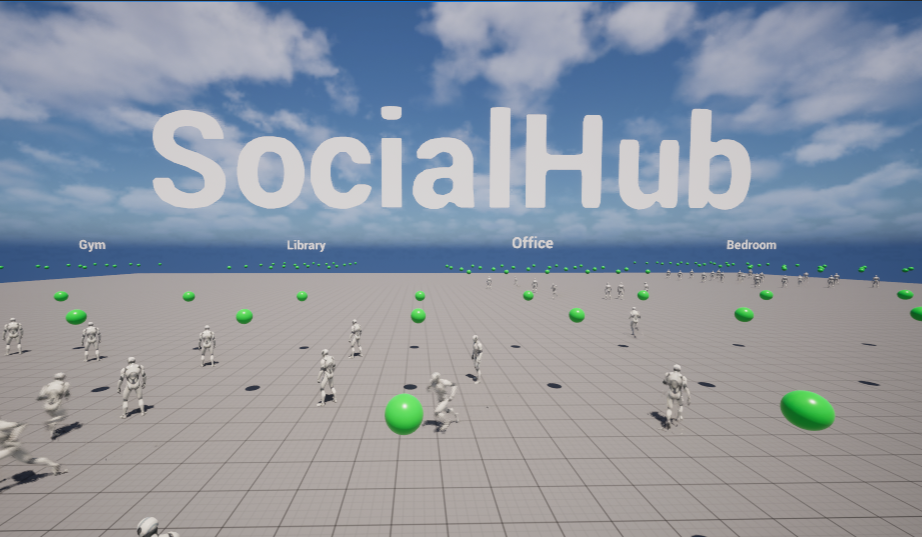
\includegraphics[width=0.95\linewidth]{ue5-topdown.png}
  \caption{\textbf{\texttt{Map\_PCSPDistrict\_M}.} Ten affordance zones
    spanning the v3 ontology (Kitchen, Bedroom, Office, Library, Gym,
    Bathroom, SocialHub, Park, Shop, Observe); each green sphere is an
    \texttt{APCSPAgentCharacter} running the hybrid \PCSP{}/BT stack.}
  \label{fig:port_map}
\end{figure}

\begin{figure}[t]
  \centering
  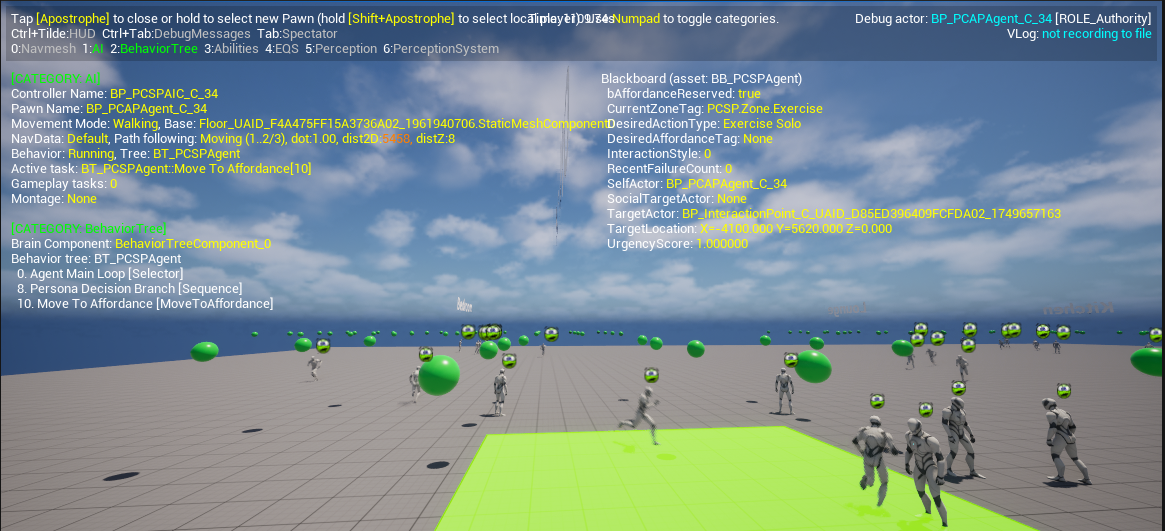
\includegraphics[width=0.95\linewidth]{ue5-x6.png}
  \caption{\textbf{Live debug overlay.} The Gameplay Debugger shows the
    Blackboard and BT state for a selected agent --- current
    \texttt{DesiredActionType}, \texttt{UrgencyScore}, active node,
    and reservation state. Same tooling a designer already uses for
    hand-authored BTs.}
  \label{fig:port_debugger}
\end{figure}

\noindent\textbf{Runtime at scale.}
A scaling sweep on a single workstation ($\{8, 16, 32, 64, 96, 128\}$
agents, 3 seeds each, $630$\,s per run) gives a clean picture of the
budget:
\begin{itemize}[leftmargin=*,nosep]
\item \emph{ONNX inference is not the bottleneck.} Mean per-call
latency stays at $\sim\!200$\,$\mu$s through $n{=}64$.
\item \emph{Frame time scales near-linearly at $\sim\!0.27$\,ms/agent.}
The $p95$ frame budget holds through $n{=}96$ ($15.9$\,ms) and goes
$0.4$\,ms over the $60$\,FPS budget at $n{=}128$.
\item \emph{NavMesh \texttt{FindPath} is the hard ceiling.} BT-abort
rate is $\leq\!0.2\%$ for $n{\leq}64$, $4.7\%$ at $n{=}96$, and
collapses to $44.9\%$ at $n{=}128$ as concurrent path queries exceed
Recast's async capacity.
\end{itemize}
The recommended operating point on a single consumer CPU/GPU is
$n{\leq}64$; $96$ is a soft cap; $128{+}$ wants async batched
pathfinding or a crowd-sim fallback. That is the single most
counterintuitive number in the project: the bottleneck is not the
neural network.

\noindent\textbf{Held-out personas, zero-shot.}
The point of a shared policy is that adding a character should be
zero training. We test this directly: train on personas $1$--$240$,
deploy on $60$ unseen personas ($241$--$300$) covering four
occupations absent from training. Result: $2{,}792$ interactions in
$9.75$\,min, $\mathbf{0.04\%}$ failure rate ($1$ stalled path of
$2{,}792$), and the inter-persona action dispersion is
\emph{slightly higher} on the unseen personas ($\rho{=}0.368$) than on
the trained ones ($\rho{=}0.383$). New characters work without retraining.

\noindent\textbf{Personality, in numbers.}
A runtime CVar (\texttt{pcsp.PolicyMode}) lets us flip between the
full policy, a zero-persona ablation, and BT-only. With the full
policy at $64$ agents: $2{,}077$ interactions, $0.0\%$ failure, action
dispersion $\rho{=}0.368$. Zero the persona embedding at inference:
dispersion collapses to $\rho{=}0.990$ (every agent behaves the
same) and failures rise to $13.3\%$ as agents synchronise on the
same most-urgent need each tick. The persona signal is not just
aesthetic; it is what \emph{desynchronises} the population enough to
keep the contention budget liveable.

\begin{figure}[t]
  \centering
  
\includegraphics[width=0.95\linewidth]{persona_persistence.pdf}
  \caption{\textbf{30 minutes of personality.} Per-minute dominant
    intent for four maximally-separated personas in UE5, frozen
    Layer-1 checkpoint, $8$ agents. Each row is one persona; each
    column is a one-minute bin coloured by the modal intent.
    \texttt{p009} stays in Rest for all $30$ bins; \texttt{p058}
    holds Work in $17/30$; \texttt{p001} cycles social-leaning;
    \texttt{p041} splits Social/Work. Training episodes are $128$
    decisions ($\sim\!2$\,min) --- the figure shows persistence over
    $\sim\!15\times$ the training horizon.}
  \label{fig:port_persistence}
\end{figure}

\noindent\textbf{Personality holds over time.}
The training episode is $128$ decision steps ($\sim\!2$\,min of
real-time play). A natural shipping question: does the personality
hold over a 30-minute session, or do agents drift into the same
behaviour as soon as the rollout exceeds what they saw at training?
Figure~\ref{fig:port_persistence} answers: \emph{no drift.} Four
maximally-separated personas hold their dominant axis end-to-end
over $30$ minutes; \texttt{p009} (rest-leaning) stays in Rest for all
$30$ minute bins. The mechanism is purely the conditioning: the
policy is stateless feed-forward and the persona embedding is frozen.

\begin{figure}[t]
  \centering
  
\includegraphics[width=0.95\linewidth]{fig_ue5_social_graph.pdf}
  \caption{\textbf{Emergent social clustering.} Co-presence graph over
    $64$ agents in a $\sim\!10$-minute session. Nodes are agents
    coloured by behavioural archetype; edges join agents who occupy
    the same zone close enough to share an interaction point. Same
    archetype clusters together (assortativity $0.36$, $63.5\%$ of
    edges same-archetype) \emph{with no social objective in
    training.}}
  \label{fig:port_social}
\end{figure}

\noindent\textbf{Bonus: emergent social structure.}
The training reward has no social term. There is no coordination
signal, no group reward, no awareness of other agents in the loss.
Yet at $64$-agent scale a co-presence graph emerges
(Fig.~\ref{fig:port_social}): agents of the same archetype cluster
together purely because their personas push them toward the same
zones at the same times. This is the kind of behaviour that takes
weeks to script in a BT, and here it falls out of the deployment
for free.

% =============================================================================
\section{Engineering Stack \& Lessons}
\label{sec:eng}
% =============================================================================

This section is the short version of what I'd tell a tech-AI lead
in a coffee chat.

\noindent\textbf{Hybrid, not end-to-end.}
End-to-end RL in a commercial engine forces a studio to throw out the
existing AI stack and re-debug from zero. The hybrid stack
($\PCSP{} \rightarrow$ intent $\rightarrow$ BT $\rightarrow$ NavMesh)
treats the policy as one well-typed decision node and leaves every
other game-AI system intact. Designers keep their BT, debugger,
EQS, and override hooks. The integration is additive.

\noindent\textbf{Inference: synchronous, throttled, no GPU required.}
ONNX runs through Epic's NNE/NNERuntimeORT plugin on the CPU path.
We call it synchronously on the BT tick with a $0.5$\,s decision
throttle and exponential backoff on repeated move failures. At $64$
agents this caps ONNX calls at $\leq\!128$/s, comfortably within
NNERuntimeORT's CPU headroom. No async batching, no GPU, no
custom plugin.

\noindent\textbf{The bottleneck is pathfinding.}
The single most counterintuitive lesson: the neural network is fast
enough; the engine's classical AI subsystems are the wall. Recast's
async query queue saturates at $n\!\sim\!96$ agents and collapses by
$n\!=\!128$. Anything past that requires either async batched
\texttt{FindPath} or a crowd-simulation fallback for the long-haul
motion. The neural part of the system gets significantly cheaper
than people expect; the physics-y bits do not.

\noindent\textbf{Persona signal as a desynchroniser.}
A subtle but important finding: removing the persona embedding at
inference doesn't just \emph{flatten} behaviour, it \emph{breaks} it.
Failure rate jumps from $0.0\%$ to $13.3\%$ because every agent
suddenly wants the same affordance at the same time. The persona
signal is doing real work for the simulation's stability, not just
for its aesthetics.

\noindent\textbf{Cost to integrate.}
Concretely, into a fresh UE5.5 project:
\begin{itemize}[leftmargin=*,nosep]
\item One \texttt{UWorldSubsystem} that owns the ONNX session and the
persona embeddings (loaded once at level start from JSON).
\item One \texttt{ACharacter} subclass with the needs/urgency
component stack.
\item Three Behavior Tree tasks: \texttt{BTTask\_PCSPDecision},
\texttt{BTTask\_MoveToAffordance}, \texttt{BTTask\_PerformInteraction}.
\item One CVar (\texttt{pcsp.PolicyMode}) for runtime ablation.
\item Per-decision JSONL trace emission, gated by a CVar.
\end{itemize}
Total: $\sim\!2{,}000$ lines of C++, one $\sim\!4$\,MB ONNX file, one
$\sim\!150$\,KB JSON. A single engineer can audit the whole stack in
an afternoon.

\noindent\textbf{Reproducibility.}
The runtime CVar makes the consistency-loss ablation re-runnable
\emph{inside the shipping engine}, not just in the research
sandbox. The same Python analyzer that processes Layer-1 trajectories
also processes UE5 JSONL traces, so paired-session statistical
comparisons (matched-persona symmetric KL) work end-to-end without
re-instrumenting.

% =============================================================================
\section{Roadmap}
\label{sec:roadmap}
% =============================================================================

\begin{itemize}[leftmargin=*,nosep]
\item \emph{Break the $n\!=\!128$ ceiling.} Move from synchronous
\texttt{MoveToLocation} to async batched \texttt{FindPath}; add a
crowd-simulation fallback for long-haul motion. Goal: $256$ agents on
the same consumer hardware.
\item \emph{Designer-facing persona tooling.} The current pipeline
is researcher-facing (Python + JSON). A designer-facing flow ---
``write a persona in the editor, hit play, see it run'' ---
turns this into something a content team can actually use without
ML knowledge.
\item \emph{Cross-substrate transfer.} The Layer-2 (Melting Pot) and
Layer-3 (UE5) checkpoints are currently separate trainings. A
single policy trained jointly across both substrates would let one
engine load the same model that handled the social-dilemma tasks.
\item \emph{Persona-aware narrative hooks.} The intent ontology is
currently $20$-d and need-driven. Extending it to narrative beats
(``Maya is now stressed about her deadline'') without retraining
is the natural next step.
\item \emph{Human evaluation at depth.} A coarse-trace pilot exists;
a full study with shipping-quality presentation (animation,
dialogue, environment) would close the loop on whether the
quantitative persona distinctness translates to perceived
personality differences.
\end{itemize}

% =============================================================================
\section*{Further Reading}
% =============================================================================

\begin{itemize}[leftmargin=*,nosep]
\item \textbf{COG 2026 paper} --- rigorous reference for theory,
ablations, and per-layer evaluation protocols.
\texttt{../cog2026\_main/main.tex}
\item \textbf{Phase-5 Melting Pot technical report} --- companion
write-up of the multi-agent substrate results.
\texttt{../../meltingpot/PHASE5\_REPORT.md}
\item \textbf{Codebase} --- \texttt{research/} (training, evaluation,
plotting) and \texttt{ue/cnzoi/} (UE5 plugin, BT, components).
\end{itemize}

\end{document}
